\documentclass[letterpaper,10pt]{article}
\usepackage[letterpaper,margin=0.75in]{geometry}
\usepackage[T1]{fontenc}
\usepackage{times}
\usepackage{amsmath,amssymb,bm,graphicx,float,booktabs,array}
\usepackage{xcolor,enumitem,tcolorbox,listings,textcomp,empheq}
\usepackage[hidelinks]{hyperref}
\setlength{\parindent}{0pt}
\setlength{\parskip}{5pt}
\setlist[enumerate]{itemsep=0.6em,topsep=0.4em}
\lstdefinestyle{mymatlab}{language=Matlab,
 basicstyle=\ttfamily\footnotesize,keywordstyle=\color{blue!70!black},
 stringstyle=\color{teal!60!black},commentstyle=\itshape\color{gray!70},
 emph={t1,y1,G1,num1,den1},emphstyle=\color{magenta}\bfseries,
 numbers=left,numberstyle=\tiny\color{gray!70},backgroundcolor=\color{gray!5},
 frame=single,showstringspaces=false,upquote=true,breaklines=true,
 columns=fullflexible,keepspaces=true,xleftmargin=1.5em,framexleftmargin=0.3em}
\lstset{style=mymatlab}
\newcommand{\RMS}{\mathrm{RMS}}
\newcommand{\dd}{\,\mathrm{d}}
\newcommand{\dochead}[1]{\begin{center}{\Large\bfseries ME 4030: Final Project}\\[5pt]
 {\large #1}\\[4pt]Quarter-Car Active Suspension\\
 Corrected public edition, September 2026\end{center}}
\newcommand{\task}[1]{\subsection*{#1}}
\newcommand{\eom}{\begin{align}
 M_s\ddot z_s&=-K_s(z_s-z_u)-C_s(\dot z_s-\dot z_u)+u,\label{eq:body}\\
 M_u\ddot z_u&=K_s(z_s-z_u)+C_s(\dot z_s-\dot z_u)-K_t(z_u-z_r)-C_t(\dot z_u-\dot z_r)-u.\label{eq:wheel}
 \end{align}}
\newcommand{\parameters}{\begin{center}\begin{tabular}{lll}\toprule
 Parameter & Value & Meaning\\\midrule
 $M_s$ & $2500\ \mathrm{kg}$ & Sprung mass\\
 $M_u$ & $320\ \mathrm{kg}$ & Unsprung mass\\
 $K_s$ & $80000\ \mathrm{N/m}$ & Suspension stiffness\\
 $C_s$ & $350\ \mathrm{N\,s/m}$ & Suspension damping\\
 $K_t$ & $500000\ \mathrm{N/m}$ & Tire stiffness\\
 $C_t$ & $15020\ \mathrm{N\,s/m}$ & Tire damping\\\bottomrule
 \end{tabular}\end{center}}

\begin{document}
\dochead{Project Handout}
\begin{tcolorbox}[colback=gray!5,colframe=gray!55,title=What to submit]
Submit one PDF containing your derivations, controller design, MATLAB code, plots,
performance tables, and discussion. Show intermediate steps and state assumptions.
Do not submit a ZIP file. Task weights are 30, 30, and 40 points.
\end{tcolorbox}
\textbf{Problem statement.} Design active suspension feedback for the quarter-car
model below. The body (sprung mass) and wheel assembly (unsprung mass) move vertically
about static equilibrium; gravity is already balanced. The actuator applies $+u$
to the body and $-u$ to the wheel. Use linear springs, viscous dampers, and an ideal
force actuator, and discuss the limitations of these assumptions.
\begin{figure}[H]\centering
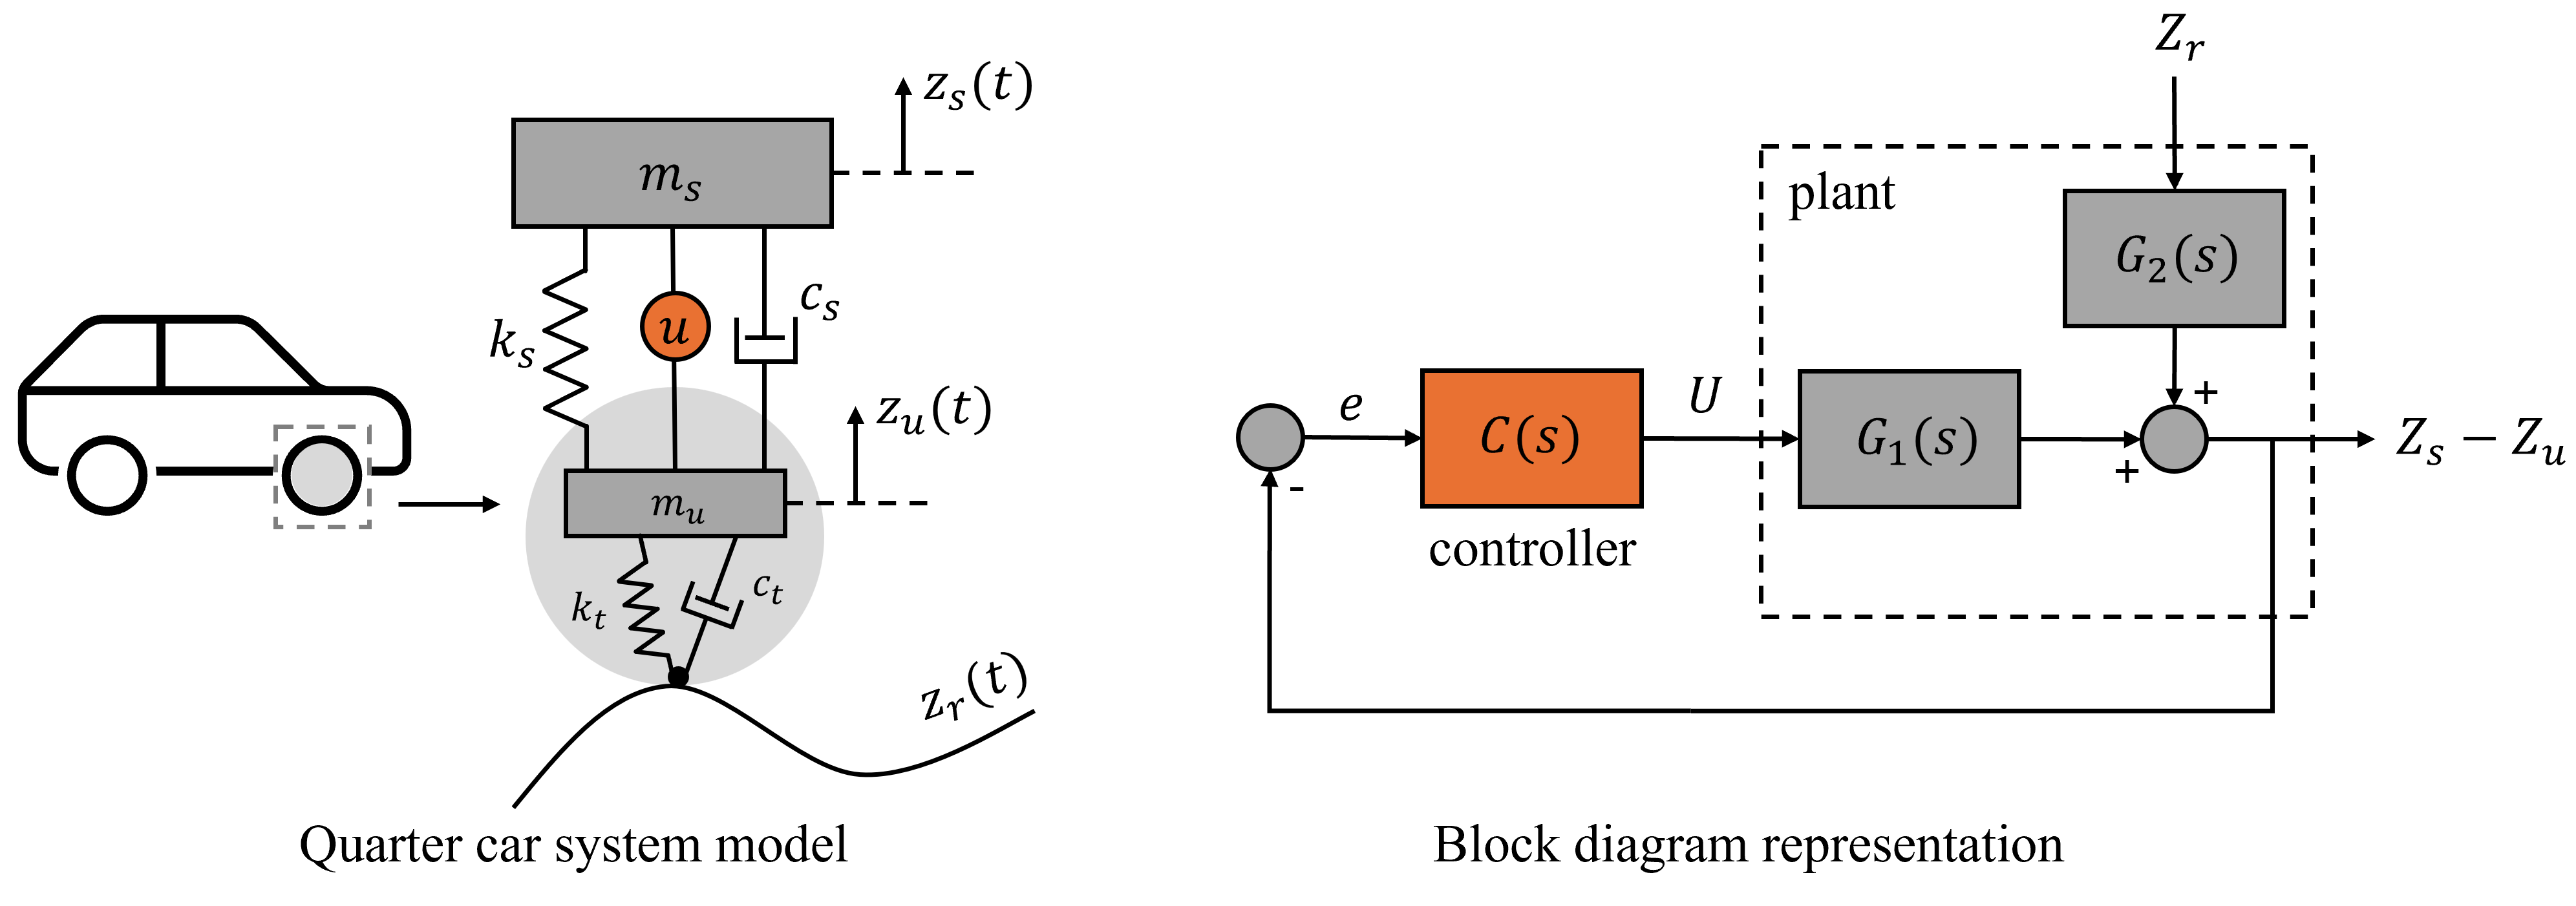
\includegraphics[width=0.61\linewidth,height=2.5in,keepaspectratio]{figures/ME4030_project.png}
\caption{Original project system diagram. Displacements share one positive direction.}
\end{figure}
\parameters
Define suspension deflection $x_s=z_s-z_u$ and tire deflection $x_h=z_u-z_r$.
The equations of motion are
\eom
Use zero initial conditions and a $T=10$ s record. Evaluate both
\begin{equation}
 z_r(t)=0.20\,\mathbf{1}_{t\geq1}\ \mathrm{m},\qquad
 z_r(t)=0.10\sin(2\pi\,0.5t)\ \mathrm{m}.
\end{equation}
An ideal road step with tire damping produces a jump in wheel velocity.
Resolve the fast transient rather than approximating the road derivative with a coarse difference.
\newpage
\section*{Performance metrics and reporting}
\begin{enumerate}
\item \textbf{Ride comfort:} absolute body-acceleration RMS,
\begin{equation}a_{\RMS}=\sqrt{\frac1T\int_0^T\ddot z_s(t)^2\dd t}.\end{equation}
This is not acceleration relative to the road.
\item \textbf{Road holding:} tire-deflection RMS,
\begin{equation}x_{h,\RMS}=\sqrt{\frac1T\int_0^T[z_u(t)-z_r(t)]^2\dd t}.\end{equation}
This linear-model proxy does not itself prove continuous tire contact.
\item \textbf{Transient performance:} for the step, report suspension recovery time:
the first time after onset beyond which $|x_s|\leq0.004$ m for the remainder of the
record. Measure from $t=1$ s. Report ``not settled'' if necessary. Percentage
overshoot relative to $x_s(\infty)=0$ is undefined.
\item \textbf{Suspension travel:} report $\max_{0\leq t\leq T}|x_s(t)|$.
\item \textbf{Control effort:} report force RMS and peak force,
\begin{equation}u_{\RMS}=\sqrt{\frac1T\int_0^T u(t)^2\dd t},\qquad
 u_{\mathrm{peak}}=\max_{0\leq t\leq T}|u(t)|.\end{equation}
Force RMS is not actuator energy; mechanical power also depends on relative velocity.
\end{enumerate}
\begin{center}\begin{tabular}{lccc}\toprule
Metric & Excellent & Good & Acceptable\\\midrule
$a_{\RMS}$ (m/s$^2$) & $\leq0.35$ & $\leq0.50$ & $\leq0.70$\\
$x_{h,\RMS}$ (m) & $\leq0.008$ & $\leq0.012$ & $\leq0.020$\\
Suspension recovery (s), step only & $\leq3$ & $\leq5$ & $\leq7$\\
$\max|x_s|$ (m) & $\leq0.015$ & $\leq0.025$ & $\leq0.040$\\
$u_{\RMS}$ (kN) & $\leq1.5$ & $\leq2.5$ & $\leq3.5$\\\bottomrule
\end{tabular}\end{center}
These are instructional design benchmarks. A single gain set need not meet all of them.
Identify unmet targets and justify tradeoffs rather than claiming feasibility without evidence.

\textbf{Supplemental body step metrics.} Report 10--90\% rise time, overshoot
$100\max(0,\max z_s-0.20)/0.20$, and settling to $0.20\pm0.004$ m.
Rise time is the difference between the first post-onset crossings of 0.02 and 0.18 m;
report unavailable crossings explicitly. The original overshoot categories (2\%, 5\%,
10\%) can be applied to \emph{body motion}, not zero-final-value suspension deflection.
Do not apply step rise, overshoot, or settling metrics to the sine run.

\textbf{Comparison table.} Make separate step and sine tables with columns for
passive, PID, LQR, and achieved target category. Include all applicable metrics above,
$K_p,K_i,K_d$, $Q,R$, and all five entries of the augmented LQR gain. State the sample
interval, integration method, and a numerical convergence check. A 1 ms plot grid can
miss significant energy in a fast PID transient; integrate squared outputs accurately.
\newpage
\task{Task 1 (30 pts): Design a PID controller}
\begin{enumerate}[label=\textbf{(\alph*)}]
\item Derive $G_1(p)=[Z_s(p)-Z_u(p)]/U(p)$ with $Z_r=0$.
Use $p$ for the Laplace variable and the output sign $x_s=z_s-z_u$ throughout.
\item Derive $G_2(p)=[Z_s(p)-Z_u(p)]/Z_r(p)$ with $U=0$.
\item Simulate the passive system ($u=0$) for both specified road inputs.
Use MATLAB and show physical body/wheel displacement and velocity, suspension
deflection, tire deflection, and road input.
\item Design negative-feedback PID control on $x_s$, with zero desired deflection.
Report $K_p,K_d,K_i$, the feedback equation, and any derivative filter.
MATLAB's \texttt{pidTuner} is optional; its reference-tracking step plot is not the
road-disturbance response. Check closed-loop stability.
\item Simulate the PID response to the 0.20 m road step and compute the metrics.
You may present several tuning sets if one set cannot meet all targets.
Discuss the force spike caused by ideal derivative action and tire damping.
\item Simulate $z_r=0.10\sin(2\pi\,0.5t)$ and discuss the PID performance using
the applicable RMS, peak-travel, and force metrics.
\end{enumerate}
\task{Task 2 (30 pts): Design an LQR controller}
\begin{enumerate}[label=\textbf{(\alph*)}]
\item Derive the physical-coordinate model with $q=[z_s,\dot z_s,z_u,\dot z_u]^T$:
\begin{equation}\dot q=\bar A q+B_u u+B_{z_r}z_r+B_{\dot z_r}\dot z_r.\end{equation}
\item Construct $x=[z_s,\dot z_s,x_s,\eta]^T$ and obtain
$\dot x=Ax+B_1u+B_2z_r$, $x_s=Cx$, eliminating the \emph{road derivative},
not the road disturbance. Use
\begin{equation}
 \alpha=\frac{C_s}{M_s}+\frac{C_s+C_t}{M_u},\qquad
 \eta=\dot x_s-\frac{C_t}{M_u}z_s+\alpha x_s+\frac{C_t}{M_u}z_r.
\end{equation}
Explain why $\eta\ne\dot x_s$. Determine stability and controllability of $(A,B_1)$.
\item Simulate the open-loop step and sine responses using the transformed model.
Recover physical wheel velocity correctly and compare with Task 1.
\item Augment with $\dot\xi=Cx$ and $x_a=[x^T,\xi]^T$. Choose $Q\succeq0$, $R>0$
and use \texttt{lqr} on the augmented plant. Report the five-entry gain, cost,
closed-loop poles, and the meaning of your weights. Explain integral action.
\item Simulate the \emph{LQR} response to the 0.20 m step and compute the metrics.
Experiment with weights and explain both achieved and unmet targets.
\item Simulate the specified sinusoidal road and compare LQR with PID and passive responses.
\end{enumerate}
\newpage
\task{Task 3 (40 pts): Performance analysis and discussion}
\begin{enumerate}[label=\textbf{(\alph*)}]
\item Analyze the ride-comfort and road-holding tradeoffs achieved by PID and LQR.
Use quantitative evidence from both disturbance cases.
\item Examine suspension travel and actuator force for both controllers. Discuss
force, speed, stroke, bandwidth, saturation, derivative filtering, and integral
windup in a practical implementation.
\item Which controller gives a more robust response to varying road disturbances,
and why? Distinguish nominal performance from robustness. Support a robustness claim
with additional tests (for example, road-frequency or mass/damping variations), or
state clearly what the two nominal simulations cannot establish.
\item Could AI or data-driven methods adjust gains or predict the road ahead in an
``autopilot'' suspension? Discuss benefits, sensing/training data, validation,
reliability, and safe fallback behavior.
\end{enumerate}
\section*{Expected learning outcomes}
By completing the project, you should be able to derive a mechanical plant and its
transfer functions; interpret transformed states and disturbance channels; implement
PID and integral-augmented LQR feedback; quantify performance and numerical error;
and communicate the compromises and practical limits of a control design.
\section*{Working files}
Start with \texttt{starter/main\_file.m}. The reference MATLAB implementation and
worked solutions are in \texttt{solutions/}; use MATLAB with Control System Toolbox.
The separate solution document follows Tasks 1--3 and includes the executable MATLAB
source in the original project's colored, numbered listing style.
\begin{tcolorbox}[colback=gray!5,colframe=gray!55,title=Corrections to the original offering]
This edition preserves the original diagram, task sequence, six PID questions,
six LQR questions, four discussion questions, and grading weights. It makes the
deflection sign consistent, corrects the auxiliary state, separates body overshoot
from suspension recovery, and corrects the LQR task's mistaken reference to PID.
The original Fall 2025 assignment dates are not deadlines for this public edition.
\end{tcolorbox}
\end{document}
